\documentclass[conference]{IEEEtran}
\IEEEoverridecommandlockouts
% The preceding line is only needed to identify funding in the first footnote. If that is unneeded, please comment it out.
\usepackage{cite}
\usepackage{amsmath,amssymb,amsfonts}
\usepackage{algorithmic}
\usepackage{graphicx}
\usepackage{textcomp}
\usepackage{xcolor}
\usepackage{footnote}
\usepackage{multicol}
\usepackage{float}
\usepackage{minted}
\usepackage{todonotes}
\usepackage{url}[hyphens]
\usepackage[acronym, nonumberlist]{glossaries}

\def\BibTeX{{\rm B\kern-.05em{\sc i\kern-.025em b}\kern-.08em
    T\kern-.1667em\lower.7ex\hbox{E}\kern-.125emX}}
\begin{document}

\title{Container workload and orchestration in high performance computing}

\author{\IEEEauthorblockN{Kees de Jong, Maxim Masterov}
\IEEEauthorblockA{\textit{SURF} \\
Amsterdam, The Netherlands \\
kees.dejong@surf.nl, maxim.masterov@surf.nl}}

\maketitle

\begin{abstract}
In e.g. federated \gls{hpc} infrastructures it is a challenge to maintain predictable software environments. Container technology offers the portability needed to keep work environments across different infrastructures consistent. Several container technologies have been developed. With container technology there is also the question of orchestration. How, where and when are these containers deployed in a  (federated) cluster? \gls{slurm} is a resource manager that is used to schedule \gls{hpc} workloads and is used in about 60\% of the \gls{hpc} infrastructures in the TOP500\footnote{\url{https://hpcc.usc.edu/support/documentation/slurm/}}. With \gls{slurm} containers may be used in job scripts or with \gls{slurm} plugins to submit jobs, allowing the scheduling of HPC workloads in containers. In Cloud environments, Kubernetes is a popular container scheduler/orchestrator. This research will investigate the pros and cons of several \gls{hpc} oriented container solutions. Furthermore, \gls{slurm} and Kubernetes will be evaluated as \gls{hpc} container schedulers.
\end{abstract}

\begin{IEEEkeywords}
SLURM, Kubernetes, Singularity, Docker, HPC
\end{IEEEkeywords}


\section{Introduction}
The use of containers in \gls{hpc} environments is gaining more popularity. Container technology is used to provide a uniform environment for testing and deploying applications. Due to the bundling of all application dependencies into one portable container, these applications provide seamless and continues updates on any container-supporting host. This provides more agility because the same environment that is used by a developer will be used on the target system. However, adoption in \gls{hpc} has been slow due to security concerns and the specific parallel \gls{rdma} application use cases on InfiniBand networks.


\subsection{Container technologies}
Several \gls{hpc} oriented container technologies have been developed and the pros and cons will be briefly summarized in this section \cite{hpc-workloads-justin, saha2018evaluation, stackhpc-state-of-hpc}.


\subsubsection{Singularity}
One of the most popular \gls{hpc} oriented container solutions is Singularity. An estimated of 25,000+ systems are running Singularity like SURF, TACC, San Diego Supercomputer Center, and Oak Ridge National Laboratory. Root privileges are not required to run and build containers.

Singularity uses \gls{sif} which is a single-image format, i.e. it does not use layers, unlike Docker. Since the \gls{oci} format supports multiple layers, they are often larger than the \gls{sif} format. \glspl{sif} are treated like a binary executable by a Linux user. However, Singularity also supports the conversion from the \gls{oci} format to \gls{sif}, which in effect allows using Docker images. Furthermore, the project enjoys active development from a broad community.


\subsubsection{Docker}
Docker is not an \gls{hpc} oriented container solution. The reason for that is that it is focused on sites with only trusted users. Docker requires root privileges to build and run containers, as also noted in the Docker documentation; ``only trusted users should be allowed to control your Docker daemon'' \cite{docker-security}. \gls{hpc} systems are in general systems where the users are not trusted with this privilege. The Docker daemon runs as root, which is considered a poor design choice in terms of security. Since Docker Engine v19.03 a new features has been introduced named rootless-mode. However, this feature is labeled as experimental and is focused on Ubuntu based systems. This rootless-mode feature also lists several known limitations \cite{docker-rootless}.

Therefore, allowing users to run Docker containers on a multi-user host with shared file systems and NFSv3 exports secured only via AUTHSYS is risky. Since users may mount these shared file systems as root and access this data. The only safe way to give users Docker like functionality on a shared host is with Singularity \cite{cloudy-hutch}.

Saha et al. researched the performance of Docker and Singularity in \gls{hpc} \cite{saha2018evaluation}. The researchers presented 1) a performance evaluation of Docker and Singularity on bare metal nodes in the Chameleon cloud 2) a mechanism by which Docker containers can be mapped with InfiniBand hardware with \gls{rdma} communication and 3) an analysis of mapping elements of parallel workloads to the containers for optimal resource management with container-ready orchestration tools. They evaluated Docker and Singularity as follows; Singularity is designed to use the underlying \gls{hpc} runtime environment for executing \gls{mpi} applications, whereas Docker is designed to isolate the runtime environment from the host. Also, Singularity focuses on coarse-grained resource allocation whereas Docker can take advantage of the fine-grained allocation of resources per rank.

The researchers performance analysis showed that scientific workloads for both Docker and Singularity based containers can achieve near-native performance. Singularity is designed specifically for \gls{hpc} workloads. However, Docker still has advantages over Singularity for use in Clouds as it provides overlay networking and an intuitive way to run \gls{mpi} applications with one container per rank for fine-grained resources allocation. Both Docker and Singularity make it possible to directly use the underlying network fabric from the containers for coarse grained resource allocation. However, Singularity provides direct support for \gls{mpi}, while Docker does not provide full support for \gls{mpi}. Docker provides more flexibility in terms of container placement with fine grained resource allocation. However, unlike Singularity, a Docker container needs to have InfiniBand interconnect drivers installed and mapped inside the container to enable fast communication. Furthermore, for \gls{mpi} applications, splitting ranks per container with restricted resources to each container can be employed by Docker. This option is not available in Singularity containers.


\subsubsection{udocker}
In response to the security concerns of Docker, several more security hardened alternatives were developed. E.g. udocker was developed, which is a Docker feature subset clone that is designed to allow execution of Docker commands without increased user privileges. udocker does not require any type of privileges nor the deployment of services by system administrators. It can be downloaded and executed entirely by the end user. udocker achieved this enhanced security functionality by executing containers completely in user space. Because of that, administrative functionality inside of the container is severely limited \cite{utah-udocker}.


\subsubsection{Charliecloud}
Charliecloud is designed to be as minimal and lightweight as possible and uses Linux user namespaces to run containers with no privileged operations or daemons and minimal configuration changes. This simple approach avoids most security risks while maintaining access to the performance and functionality already on offer. Charliecloud was not deemed stable enough for \gls{rhel} due to the dependence on kernel namespaces in 2017 \cite{kurtzer2017singularity}. However, \gls{rhel} 8 is shipped with Podman (Red Hat's own container solution), which also makes use of kernel namespaces. It does not require root privileges to install the Charliecloud software or to run Charliecloud containers.


\subsubsection{Podman}
Podman was developed by Red Hat as a root-less container solution. It is designed without the overhead and security concerns of the full Docker daemon. Currently Podman is not entirely suitable for \gls{hpc} use cases;
\begin{itemize}
    \item Missing support for parallel filesystems (e.g. IBM Spectrum Scale).
    \item Rootless Podman was designed to use kernel user namespaces which is not compatible with most parallel filesystems.
    \item Not yet possible to set system wide policy defaults.
    \item Pulling and building Docker/OCI images requires manual subuids/subgids entries for each user.
\end{itemize}
Buildah offers a promising way to enable users to build container images as Docker/OCI images, all without root privileges.


\subsubsection{Shifter}
Shifter is mostly backed by the \gls{nersc} and Cray. Documentation uses \gls{slurm} for job scheduling. However, instead of the \gls{oci}, Shifter uses their own format, which is reverse-compatible with the \gls{oci} format. Community support lacks for Shifter, other than \gls{nersc} and Cray there are not many other contributors, which indicates low engagement of the \gls{hpc} community. This translates in low development activities, a pull request for better \gls{mpi} integration, which was opened in April 2017, has since stalled.


\subsubsection{Enroot}
Enroot can be thought of as an enhanced unprivileged chroot. It uses the same underlying technologies as containers but removes much of the isolation they inherently provide while preserving filesystem separation. This approach is generally preferred in \gls{hpc} environments or virtualized environments where portability and reproducibility is important, but extra isolation is not warranted.

Enroot is also similar to other tools like proot or fakeroot but instead relies on more recent features from the Linux kernel (i.e. user and mount namespaces), and provides facilities to import well known container image formats (e.g. Docker). Furthermore, it does not require a daemon or extra process. Several advanced features include; runfiles, scriptable configs, and in-memory containers \cite{nvidia-slurm-containers}. Root privileges are required to build containers with enroot. However, Buildah from Red Hat may be used to build containers as well which can then be converted to the enroot format.


\subsection{Container orchestrators}
\subsubsection{SLURM}
\gls{slurm} provides the means to allocate exclusive and/or non-exclusive access to typically \gls{hpc} compute resources for a duration of time. Therefore, \gls{slurm} provides a scheduling framework for starting, executing, accounting and monitoring compute jobs. These are typically parallel \gls{mpi} jobs on a set of scheduled compute nodes, or parallel OpenMP jobs on a single scheduled compute node. \gls{slurm} also provides the intelligence to manage queues and thus congestion of the compute resources. \gls{slurm} is also topology-aware, which is the intelligence to schedule jobs on nodes close together in the \gls{hpc} cluster in order to keep latency low. The \gls{hpc} use case consists of parallel compute jobs with a defined, relative short runtime. \gls{slurm} is generally agnostic towards container technologies and start most, if not all.

\subsubsection{Kubernetes}
Kubernetes has risen to the top in the challenge to provide orchestration and management for containerized software components due to its rich ecosystem and scaling properties. Kubernetes provides portability, ease of administration, high availability, integrability, and monitoring capabilities for container orchestration. While \gls{hpc} workload managers are focused on running distributed memory jobs and support high-throughput scenarios, Kubernetes is primarily built for orchestrating containerized microservice applications and has grown popular in e.g. Cloud-native workloads, high-throughput computing and data analytics workflows. These microservices require resilience, which Kubernetes provides with load-balancing and redundancy features. In order to provide the maximum availability over a relative long lifespan,  microservices are updated and maintained while in production \cite{hpc-kubernetes-containers}, in contrast to \gls{hpc} jobs which have a relative short and static lifespan.





% TODO: highlight the importance of the overlay network in kubernetes
% todo: what container types does kubernetes support?
% todo: which container types does slurm support? https://slurm.schedmd.com/containers.html


\subsection{Summary}
In this section we have introduced the reader with the different container technologies and two orchestrators. It was pointed out that Docker is not ideal for \gls{hpc} environments since it requires trusted users. udocker showed significant progress in terms of security by running containers fully in userspace, however, this limited its functionality. Charliecloud is a secure container solution with a small attack surface due to its lightweight nature. Charliecloud also does not require root privileges to build and run a container. Podman shows much promise due to its ability to also build and run containers without root privileges and much overhead. However, at the time of writing this report, Podman lacks the \gls{hpc} oriented features. Shifter lacks community support and its current development activities are too low to pursue it further. Singularity is a secure and very popular container solution which allows to build and run containers without root. Enroot has a different approach, the project mixes different isolation methods, while staying lightweight, with builtin GPU support.

% Figure \ref{fig:container-tech} was taken from the proceedings of the \gls{slug} meeting in 2019 and illustrates the weaknesses and strengths of several of the discussed container technologies \cite{nvidia-slurm-containers}.

% \begin{figure}[H]
% \centering
% 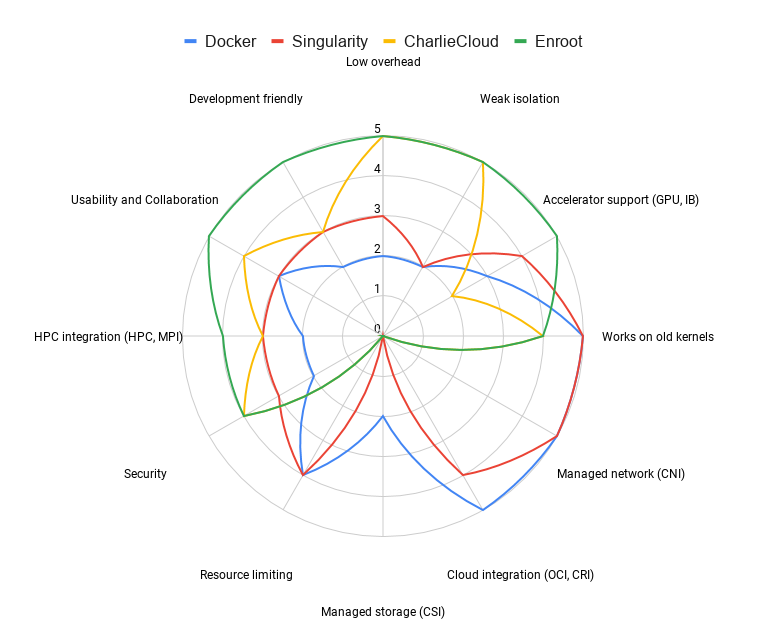
\includegraphics[width=\columnwidth]{images/container_tech.png}
% \caption{Container technology comparison}
% \label{fig:container-tech}
% \end{figure}

The two container orchestrators discussed in this section can be summarized as follows. \gls{slurm} is focused mainly on scheduling a distributed parallel compute job with a defined wall clock time. Where it is specialized in customizable efficient partitioning, queuing, accounting, monitoring and prioritizing jobs while being topology-aware. While Kubernetes is mainly focused on keeping microservices up and running without interruption. Where it is specialized with redundancy features where for instance a new instances of a container is spawned when failures occur (high availability). And load-balancing features between containers to prevent congestion and latency for the microservice. There are developments towards support for HPC workflows. However, Kubernetes still lacks the features to fully support these HPC workflows on an equivalent level as \gls{slurm}.

% Figure \ref{fig:kube_vs_slurm} was taken from the proceedings of the \gls{slug} meeting in 2019 and illustrates the weaknesses and strengths of \gls{slurm} and Kubernetes, however, container support has since been added to \gls{slurm}, thus this illustration from nVidia is as of writing this report not entirely up to date anymore \cite{nvidia-slurm-containers}.

% \begin{figure}[H]
% \centering
% 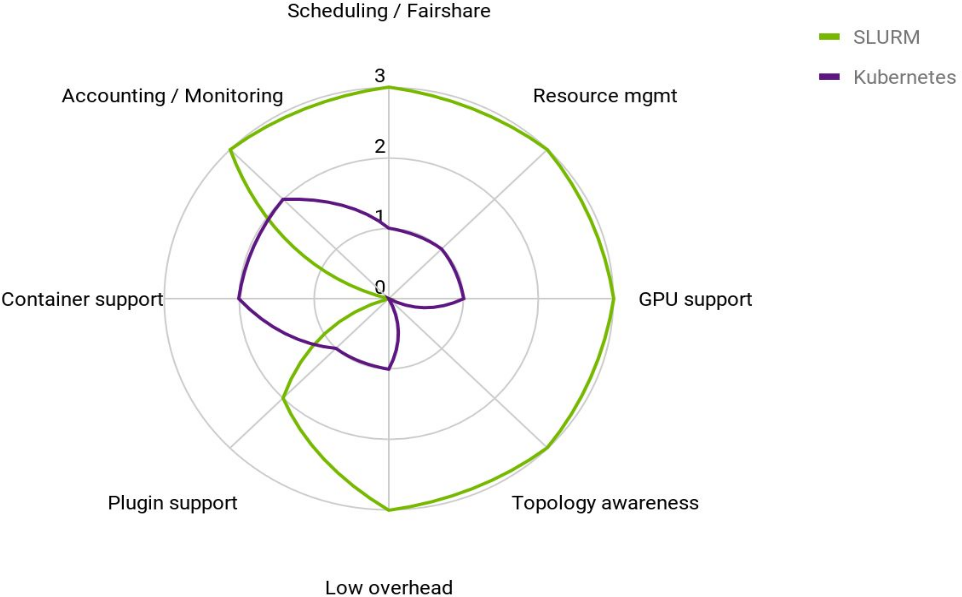
\includegraphics[width=\columnwidth]{images/hpc_vs_data_science.png}
% \caption{Kubernetes versus SLURM}
% \label{fig:kube_vs_slurm}
% \end{figure}


% \section{Related work}
% % todo: find more info about slurm + container orchestration
% \subsection{Orchestrators performance}


\section{Research question}
\label{research-question}
The following research questions are formulated and tested. How do these container technologies compare in therms of usability, security, features, and performance on single and multi node compute jobs? Furthermore, how to orchestrate/schedule compute jobs with containers? How do Kubernetes and \gls{slurm} compare with each other in terms of usability, scheduling features, features, and resource allocation?
% For Kubernetes, for example it needs to be determined if Weave-Net is the appropriate network plugin for the cluster. A
% comparison of network plugins for Kubernetes in conjunction with OpenMPI would be a
% great point of future research. Another way that Kubernetes cluster could be optimized is
% by moving from SSH to RSH for fenced networks. This same optimization could be
% applied to Beowulf clusters as well.

% Another way that Kubernetes cluster could be optimized is
% by moving from SSH to RSH for fenced networks.

% One additional optimization for Kubernetes would be to create a static, custom pod as the
% front-end node. Once the custom pod is provisioned then the batch job would select the
% front-end node instead of creating new pods each time. Provisioning all pods including
% the front-end pod ahead-of-time would eliminate most of the startup time.


\section{Method}
In order to answer the research question from section \ref{research-question}, we tested \todo{maxim: define jobs and what they test} x, y, z jobs on single and multi node jobs and measured the performance x times. These performance metrics were visualized in box plots to demonstrate the performance stability compared to bare metal performance. Furthermore, the usability, security and features of the container technologies were visualized in spider graphs. We did not setup a Kubernetes cluster due to the sufficient related work available. The evaluation of Kubernetes and \gls{slurm} was a literature study of which the results were also visualized in spider graphs. These spider graphs of the container technologies and container orchestrators visualize the pros and cons of each solution. 


\section{Results}
In this section the container benchmark results are evaluated. The container orchestrators are evaluated exclusively based on related work.

\subsection{Container technologies}
% Results discussed here
% * What can be concluded here? Try to make it a bit more broader then "they are similar", something like; even though of the extra overhead the performance is ... bla bla
% * by looking at the boxplots, the performance is very stable, no outliers and the min and max values of the quartiles are tight

% I will split this up in some smaller figures for it to fit better in column space. but in the meantime the text can be written already
\begin{figure*}
\centering
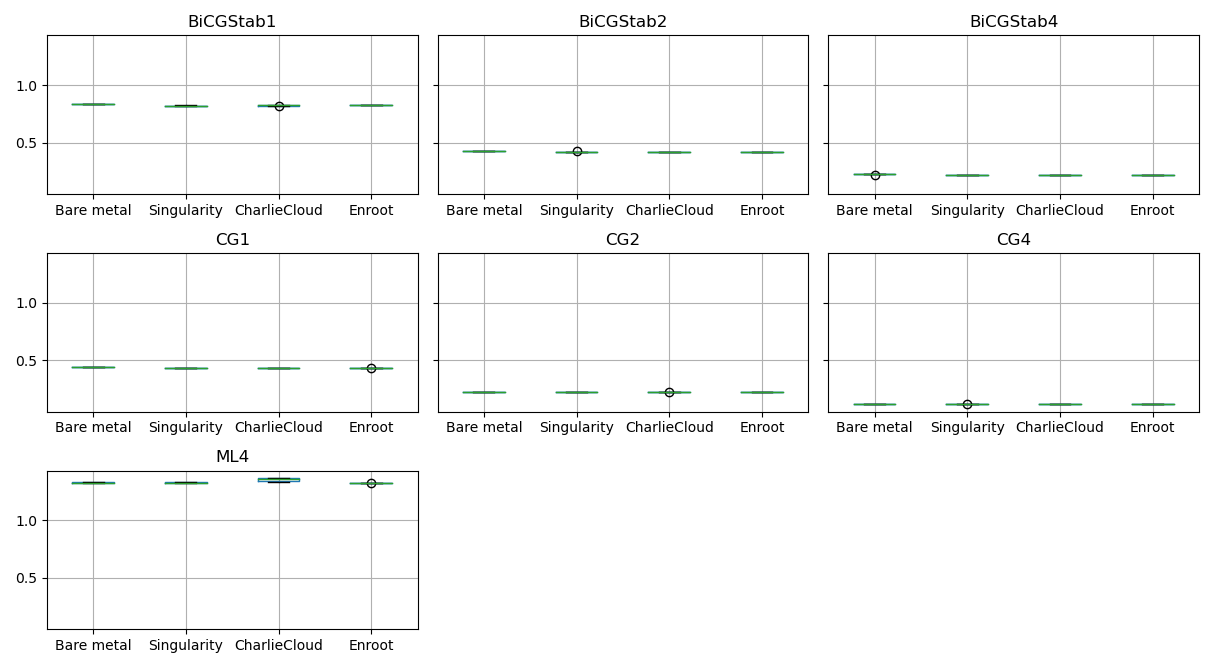
\includegraphics[width=\textwidth]{images/container_benchmarks.png}
\caption{Container technology benchmarks}
\label{fig:container_benchmarks}
\end{figure*}



\subsection{Container orchestrators}
Futral researched the performance differences of several batch schedulers, including \gls{slurm} and Kubernetes \cite{futral2019method}. The research's measurements were wall clock time, RAM usage, and CPU usage. These measurements captured the utilization of system resources for each of the schedulers. The batch jobs were composed of custom scripts, using the NASA Parallel Benchmark programs and computational fluid dynamics, which were executed using, 1, 2, and 4 servers to determine how well a scheduler scales with network growth. All hardware was similar and was co-located within the same data-center.

Kubernetes performed less than \gls{slurm}. For instance, Kubernetes needed to determine if Weave-Net was the appropriate network plugin for the cluster before starting a container. This overhead resulted in a slower time-to-spool. Furthermore, Kubernetes did not perform well because the worker pods had to be first provisioned before a controller pod could be provisioned via the batch job. The batch job then had to perform a DNS lookup of the worker pods and then it would be forced to wait till the worker pods were available. Kubernetes also consumed the most RAM. Furthermore, the Kubernetes cluster also suffered from utilizing SSH for its communication protocol. In addition to SSH, the researcher's Kubernetes setup also relied on a virtual network and custom dynamic DNS solutions to determine worker node availability. The added layer of the virtual network and the DNS lookups significantly affected Kubernetes' its performance.

\gls{slurm} performed best and did not appear to require any optimizations in terms of additional configuration of the supporting OpenMPI libraries themselves.

While Kubernetes does provide some batch job facilities, ease of development, and process isolation; the researcher concluded that it did not perform as well as expected overall. In conclusion, the data that was collected suggests that most batch schedulers are uniquely tuned to improve performance of high-performance compute jobs. This advanced tuning was especially pronounced in \gls{slurm} and Portable Batch Scheduler, but was less pronounced with Kubernetes.

"Embarrassingly parallel", or "perfectly parallel" applications on a Kubernetes cluster can indeed launch multiple containers in parallel, but the scale is "best effort" at launch time as "gang scheduling" is not possible; also it is not possible for the application to perform different functions on the "primary" container as the "secondaries", so sharding and setup must be performed either in advance or manually. This is not architecturally compatible with most existing applications \cite{hpc-on-kubernetes}.

A Kubernetes cluster is not suitable as a tightly-coupled parallel solver as it cannot guarantee scale neither at launch nor at runtime, does not support “gang scheduling” to queue jobs until all parallel resources are available, does not automatically elect and run code on a "primary" node, and does not automatically configure fabric for applications.

Accelerated parallel training for AI is not supported for the same reasons as for parallel solvers; alternative training
workflows must be used (assuming framework support) when scale is needed. However, AI support for accelerated real-time analytics is supported assuming Kubernetes plugins exist for accelerated hardware, it may support these stacks.

Many \gls{hpc} applications have specific requirements relative to where they are executed within the system. Where each task (rank) of an application may need to communicate with specific neighboring tasks and so prefer to be placed topologically close to these neighbors to improve communication with these neighbors. Other tasks within the application may be sensitive to the performance of the I/O subsystem and as such may prefer to be placed in areas of the system where I/O throughput or response times are more favorable \cite{stackhpc-kubernetes-mpi}.

There are projects underway with the goal of integrating Kubernetes with MPI. One notable approach, kube-openmpi, uses Kubernetes to launch a cluster of containers capable of supporting the target application set. Once this Kubernetes namespace is created, it is possible to use kubectl to launch and mpiexec applications into the namespace and leverage the deployed OpenMPI environment. kube-openmpi only supports OpenMPI, as the name suggests.

Another framework, Kubeflow, also supports execution of MPI tasks atop Kubernetes. Kubeflow’s focus is evidence that the driving force for MPI-Kubernetes integration will be large-scale machine learning. Kubeflow uses a secondary scheduler within Kubernetes, kube-batch to support the scheduling and uses OpenMPI and a companion ssh daemon for the launch of MPI-based jobs. Such approaches do not fully leverage the flexibility of the elastic Kubernetes infrastructure, or support the critical requirements of large-scale HPC environments, as described above.

In some respects, kube-openmpi is another example of the fixed use approach to the use of containers within HPC environments. For the most part there have been two primary approaches. Either launch containers into a conventional HPC environment using existing application launchers (e.g., Shifter, Singularity, etc.), or emulate a conventional data parallel HPC environment atop a container deployment (à la kube-openmpi).

Furthermore, Kubernetes 1.18 enables a new feature called Topology Manager \cite{gridengine-topology}. This is a component of Kubelet which also takes care of NUMA optimizations, which runs locally on the target host. Topology Manager provides a host local logic, which enables; 1) only host local decisions and 2) lead to wasted resources when pods needs to be re-scheduled many times to find a host which fits. The Topology Manager provides following allocation policies: none, best-effort, restricted, and single-numa-node. These are kubelet flags. The actual policy which is applied to the pod depends on the kubelet flag but also on the QoS class of the pod itself. The QoS class of the pod depends on the resource setting of the pod description. If CPU and memory are requested in the same way within the limits and requests section then the QoS class is guaranteed. Other QoS classes are BestEffort and Burstable. The kubelet calls so called Hint Providers for each container of the pod and then aligns them with the selected policy, like checking if it works well with single-numa-node policy. When set to restricted or single-numa-node it may terminate the pod when no placement if found so that the pod can be handled by external means (like rescheduling the pod).

Some interesting development efforts and functionalities already in place for Kubernetes \cite{kubecon-2018}.
\begin{itemize}
    \item CRI-O lightweight container runtime + rootless usage
    \item CPU Pinning and Isolation
    \item Device Plugins (GPUs, Infiniband, FPGA, etc)
    \item NUMA Management
    \item SR-IOV Networking plugin
    \item Spark 2.3.0 with Kubernetes scheduler instead of Yarn
    \item Pods Priorities and Preemption
    \item Container Runtime
        \begin{itemize}
        \item CRI-O - OCI stable runtime follow rootless
        \item KataContainers - OCI VM Containers
        \item Singularity - Syllabs seems to be working on support of Kubernetes
        \item Gvisor - Google sandboxed containers
    \end{itemize}
    \item Kubernetes cluster federation – for offloading on hybrid clouds
    \item Kubeflow to make Machine Learning simple, portable and scalable
\end{itemize}

The Kubernetes blog provides several suggestions for HPC deployments \cite{kubernetes-blog-hpc}. 1) Maintain separate infrastructures. For sites with sunk investments in HPC, this may be a preferred approach. Rather than disrupt existing environments, it may be easier to deploy new containerized applications on a separate cluster and leave the HPC environment alone. The challenge is that this comes at the cost of siloed clusters, increasing infrastructure and management cost.

2) Run containerized workloads under an existing HPC workload manager. For sites running traditional HPC workloads, another approach is to use existing job submission mechanisms to launch jobs that in turn instantiate containers on one or more target hosts. Sites using this approach can introduce containerized workloads with minimal disruption to their environment. Leading HPC workload managers such as Univa Grid Engine Container Edition and IBM Spectrum LSF are adding native support for containers. Shifter and Singularity are important open source tools supporting this type of deployment also. While this is a good solution for sites with simple requirements that want to stick with their HPC scheduler, they will not have access to native Kubernetes features, and this may constrain flexibility in managing long-running services where Kubernetes excels.

3) Use native job scheduling features in Kubernetes. Sites less invested in existing HPC applications can use existing scheduling facilities in Kubernetes for jobs that run to completion. While this is an option, it may be impractical for many HPC users. HPC applications are often either optimized towards massive throughput or large scale parallelism. In both cases startup and teardown latencies have a discriminating impact. Latencies that appear to be acceptable for containerized microservices today would render such applications unable to scale to the required levels.


\section{Conclusion}
Traditional HPC and Kubernetes Co-Existence Is it possible? Yes, but I wouldn’t recommend it on a shared HPC cluster \cite{cloudy-hutch}.

While Kubernetes excels at orchestrating containers, \gls{hpc} applications can be tricky to deploy on Kubernetes \cite{kubenetes-blog-meets-hpc}.


Kubernetes is not designed for \gls{hpc} hence it will never be as optimized as \gls{slurm}. However, In the effort to enable support of Big Data and Artificial Intelligence the software is being enhanced with functionalities that will eventually interest the \gls{hpc} community. Furthermore, the convergence of \gls{hpc} and Big Data will further motivate the usage of Kubernetes in \gls{hpc}.

% SLURM NOTES

% Advanced scheduling algorithms (fair-share, backfill, preemption, hierarchical quotas)
% Gang scheduling: scheduling and starting all processes of a multi-node job simultaneously
% Low runtime overhead
% Topology-aware (NUMA/PCIe) job scheduling for better performance
% Simple CLI with jobs as bash scripts
% GPUs are a first-class resource
% Supports interactive jobs
% Slurm does not support containers out of the box... but is extensible through plugins


\newacronym{slurm}{SLURM}{Simple Linux Utility for Resource Management}
\newacronym{cca}{CCA}{Central Converged Architecture}
\newacronym{hpc}{HPC}{High Performance Computing}
\newacronym{mpi}{MPI}{Message Passing Interface}
\newacronym{cola}{COLA}{Customer Organisation LDAP Accounting Service}
\newacronym{rdma}{RDMA}{Remote Direct Memory Access}
\newacronym{rhel}{RHEL}{Red Hat Enterprise Linux}
\newacronym{oci}{OCI}{Open Containers Initiative}
\newacronym{nersc}{NERSC}{National Energy Research Scientific Computing Center}
\newacronym{sif}{SIF}{Singularity Image Format}
\newacronym{slug}{SLUG}{SLURM User Group}

\bibliographystyle{./bibliography/IEEEtran}
\bibliography{./bibliography/IEEEabrv,./bibliography/IEEEexample}

\end{document}